\documentclass[12pt]{article}

\usepackage[english]{babel}
\usepackage[utf8x]{inputenc}
\usepackage{amsmath}
\usepackage{graphicx}
\usepackage[colorinlistoftodos]{todonotes}
\usepackage{listings}
\usepackage{color}
\usepackage{indentfirst}

\definecolor{nGreen}{rgb}{0,0.6,0}
\definecolor{nGray}{rgb}{0.5,0.5,0.5}
\definecolor{nPurple}{rgb}{0.58,0,0.82}
\lstset{ 
  backgroundcolor=\color{white},   
  basicstyle=\footnotesize,       
  breakatwhitespace=false,         
  breaklines=true,                
  captionpos=b,                  
  commentstyle=\color{nGreen},   
  extendedchars=true,             
  frame=false,	                 
  keepspaces=true,                 
  keywordstyle=\color{blue},       
  language=C,                 
  numbers=left,                   
  numbersep=5pt,                  
  numberstyle=\tiny\color{nGray}, 
  rulecolor=\color{black},        
  showspaces=false,               
  showstringspaces=false,         
  showtabs=false,                 
  stepnumber=1,                   
  stringstyle=\color{nPurple},    
  tabsize=2,	                  
  title=\lstname                  
}

\title{Creating a Linux Kernel Module (LKM) using C to interact with Arduino}
\author{Arturo Chinchilla Sánchez, Malcolm Davis Steele}
\begin{document}
\maketitle
%------------------------------------------------------------------------------------------
% 	ABSTRACT
%------------------------------------------------------------------------------------------
\begin{abstract}
  As part of the course Languages, Compilers and Interpreters, will be created a LKM for Linux 3.x which will be written in pure C and interact with an Arduino device.
  “A loadable kernel module (LKM) is a mechanism for adding code to, or removing code from,
  the Linux kernel at run time. They are ideal for device drivers, enabling the kernel to
  communicate with the hardware without it having to know how the hardware works. The
  alternative to LKMs would be to build the code for each and every driver into the Linux kernel.
  Without this modular capability, the Linux kernel would be very large, as it would have to
  support every driver that would ever be needed on the system. You would also have to rebuild
  the kernel every time you wanted to add new hardware or update a device driver. The
  downside of LKMs is that driver files have to be maintained for each device. LKMs are loaded
  at run time, but they do not execute in user space — they are essentially part of the kernel."\cite{Molloy}
\end{abstract}
%----------------------------------------------------------------------------------------

%----------------------------------------------------------------------------------------
%	CONTENTS AND FIGURES
%----------------------------------------------------------------------------------------
\newpage
\tableofcontents % Prints the main table of contents
\listoffigures % Prints the list of figures

%----------------------------------------------------------------------------------------
%  INTRODUCTION
%-----------------------------------------------------------------------------------------
\newpage
\section{Introduction}

Linux was originally developed by Linus Torvalds in 1991 to be a operating system for the IBM Personal computers, it's a Unix-Like operating system. The Linux Kernel is widely known for his flexibility and the power that grants to the programmer, this because even though his source code is big, it can be modified with all the tweaks that are looked for. One way to do this is with a Loadable Kernel Module or LKM. This is a piece of code that can be loaded to the Linux kernel so you can add functionality to the system \cite{Hartman07}.

LKMs are written in C programming language, this language was developed in the Bell Labs(AT\&T), and one of his purposes was to develop the Unix kernel. "By early 1973, the essentials of modern C were complete. The language and compiler were strong enough to permit us to rewrite the Unix kernel for the PDP-11 in C during the summer of that year" \cite{Ritchie}.

For writing a LKM some specific headers for the kernel modules like the \emph{"linux/module.h"} or the \emph{"linux/module.h"} are included to the code, then the functions that the kernel will perform. Two important methods that the LKM must have are the one that loads the module to the kernel and the one that cleanup the module and dereference it, this methods can be named as the programmer wants if he specifies with the \emph{"module\_init(methodName)"} and the \emph{"module\_exit(methodName)"} functions. If not also can be used the default names \emph{"init\_module"} and \emph{"cleanup\_module"}.

The LKM after been written, can be compiled and inserted to the Linux with the make command on a terminal located on the same place as the \emph{"module.c"} file, then you can insert the module with \emph{"insmod module.ko"}. When the module is inserted the  \emph{"init\_module"} method will be called, and after that module you can list the active modules with the method \emph{"lsmod"} or show the module info with \emph{modinfo module} , finally when up to clean the module from kernel, it's used the command \emph{"rmmod module"}. Some of this commands needs root rights to use them so with the word sudo before the command the module is up to go\cite{Henderson06}. An example code of a hello world module with his corresponding make file will be as follows.
%---------------------------------------------------------------------------------------
% 		CODE EXAMPLES
%---------------------------------------------------------------------------------------
\lstinputlisting[caption=Hello World Module \cite{Salzman-Burian-Pomerantz}]{Code/hello-2.c}
\lstinputlisting[caption=Makefile \cite{Salzman-Burian-Pomerantz}]{Code/Makefile}


The LKM can be used for many purposes, but the most common are device drivers, file system drivers, network drivers and system calls.\cite{Henderson06} As the main function is to communicate the hardware with the user space, the most uses are implementation of drivers. 

The Arduino hardware consists of a printed circuit board with a micro-controller, usually Atmel AVR (in this case Atmega328), and digital and analog input / output, which can be connected to expansion boards (shields) that expand the features operation of the Arduino.
Arduino platform provides its own language, for programming the same, which is very easy to learn and has its own functions to handle the Arduino in a more correct way, , also has its own IDE, which provides very useful characteristics; for interaction with the same, so very rare to see someone wants to program your arduino in a different language as is C, this causes the documentation is very sparse. Not having enough required documentation, it is taken as a reference Data Sheet micro-controller (Atmega328) which indicates how to manipulate all pins of the Arduino, which is a task a little tangled, for the impressive amount of codes for setting each one of the functions of each pin.
\section{Development environment}
\subsection{Overleaf:}
Free online tool used to write academic documents. This service allow create, edit and share your documents easily using \LaTeX. Provide two principal windows, in the first you can write your document, obviously using the \LaTeX syntax, and the second you can see your compiled document. \LaTeX also is composed of a large set of macros getting documents have a typographic high quality. Therefore it is widely used for the creation of academic papers, theses and technical books, since the typographic quality and made with \LaTeX documents is comparable to that of a great scientific publishing. The source can be found on \cite{Chin-Dav16a}. Fig 1.
\begin{figure}[h!]
 	\centering
  	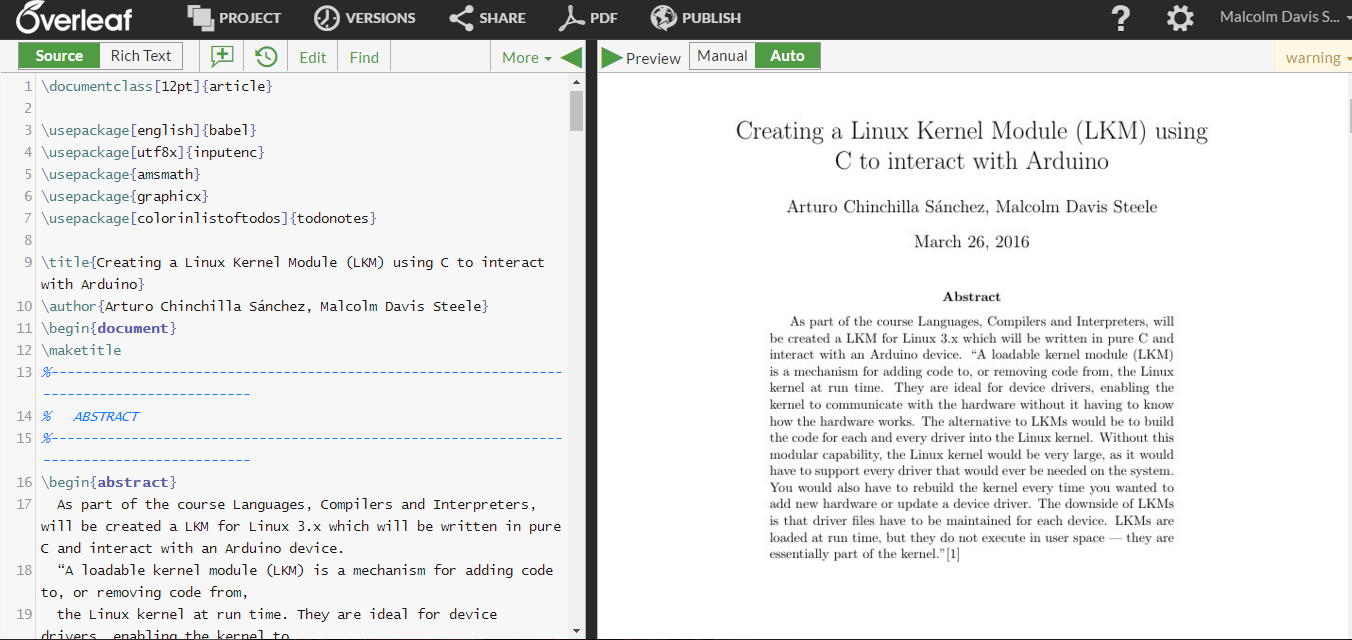
\includegraphics[scale=0.4]
  	{Fig/Inception.png}    
  	\caption{Overleaf Project.}
\end{figure}
\subsection{Git and GitHub:}
To store the code in a practical way and have a versioning control Git is used  for creating repositories and GitHub as service and cloud storage. This code manager (Git) let us to create branches for each member of the group and work separately, change the branch work, see and edit code of another branches, make commits for later if you want to go back in your code and when each part needed is done they can be merged into master branch to have a final version of the code. The code can be found on \cite{Chin-Dav16b}. Fig 2.
\begin{figure}[h!]
 	\centering
  	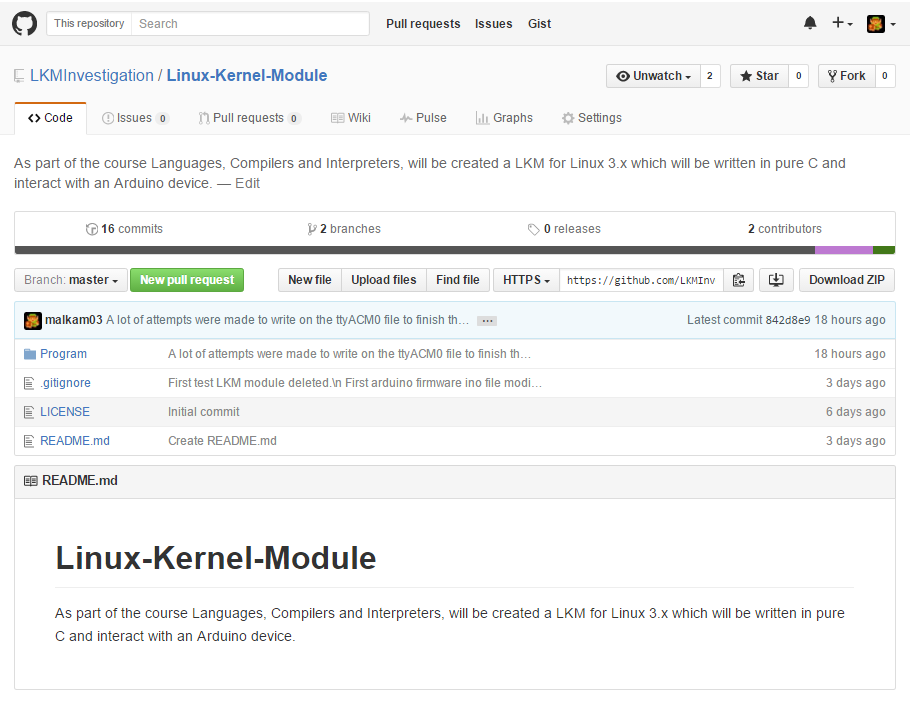
\includegraphics[scale=0.5]
  	{Fig/git.png}    
  	\caption{Git Project Home.}
\end{figure}
\subsection{123D Circuits}
This tool it's useful for sketch the circuits of a short project, and can be used to simulate the circuits and the program on the arduino(just arduino code). Also the circuit can be viewed in 3 different modes and design a PBC board. It was used for the Arduino-Led Circuit and for simulate the code before flashing the arduino. Fig 3. 
\begin{figure}[h!]
 	\centering
  	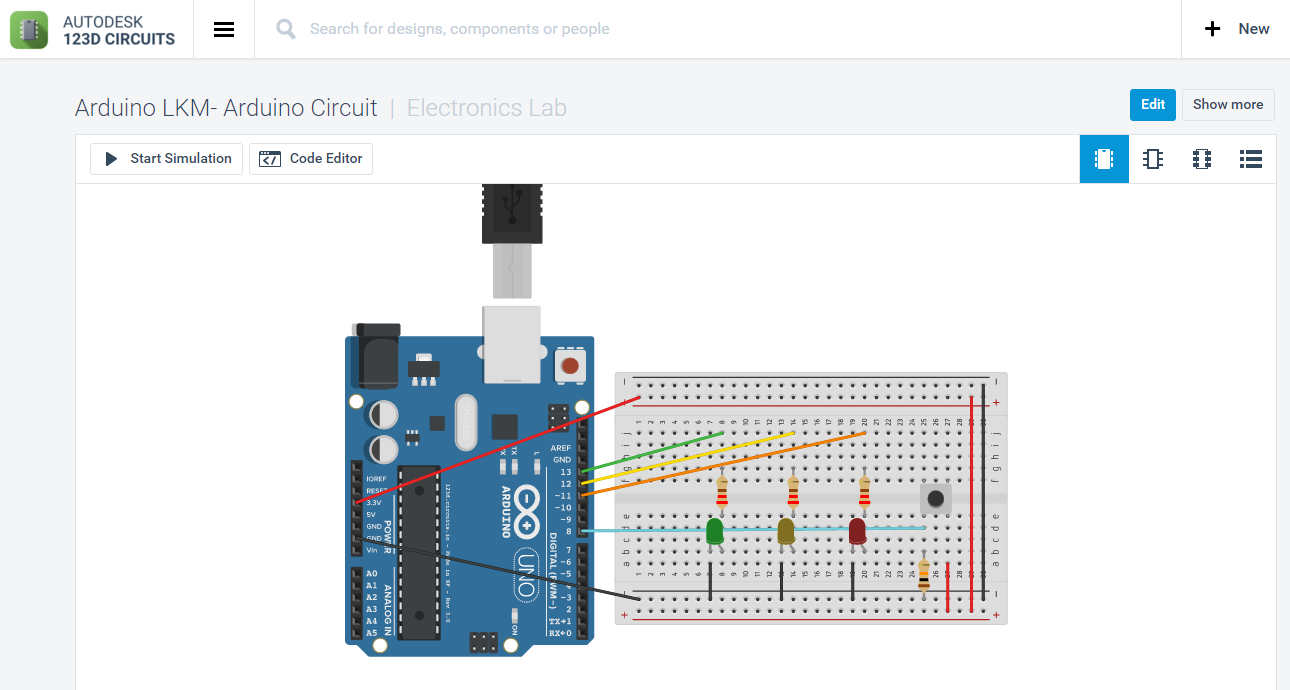
\includegraphics[scale=0.4]
  	{Fig/123D-Circuits.png}    
  	\caption{123D Circuit Home.}
\end{figure}
\subsection{Sublime Text:}
It's a text editor for code, markup and prose. It contain functionalities very  useful for programmers and facilitate the code development process. It proved to be very versatile and stable, giving good impressions, simple but with great features. Things like word suggestion, coloring restricted words, minimap, multi selection and multi cursor.Also support multiple languages like Java, C, C++ and others. Fig.\ref{Sublime}
\begin{figure}[h!]
 	\centering
  	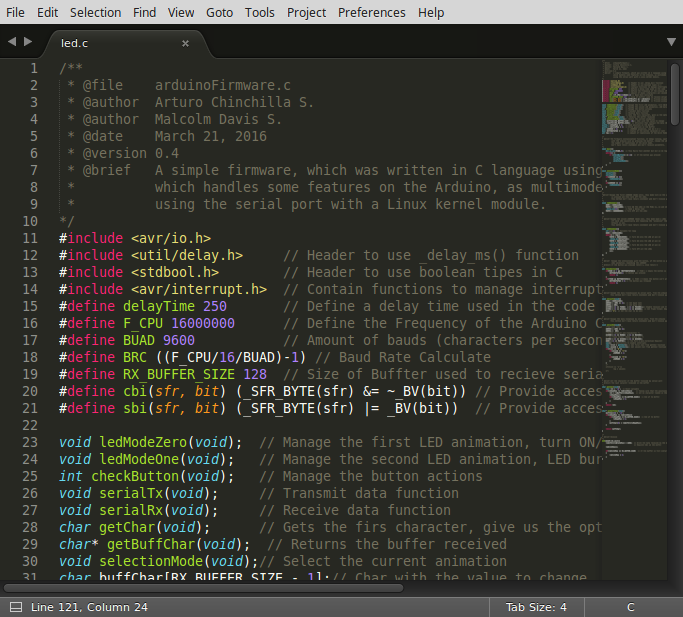
\includegraphics[scale=0.4]
  	{Fig/Sublime_Text.png}    
  	\caption{Sublime Text, text editor.}
    \label{Sublime}
\end{figure}

\section{Data Structures, functions and libraries}
Provide a description of all the functions, libraries and data structures used for the development of this project.
\section{Instructions to use each of the programs}
Before using the program it's needed to have the hardware requirements, for this project the Arduino Uno it's used, but can be used with other arduino types. The circuit of the arduino used is the one of the Fig. 5.
\begin{figure}[h!]
 	\centering
  	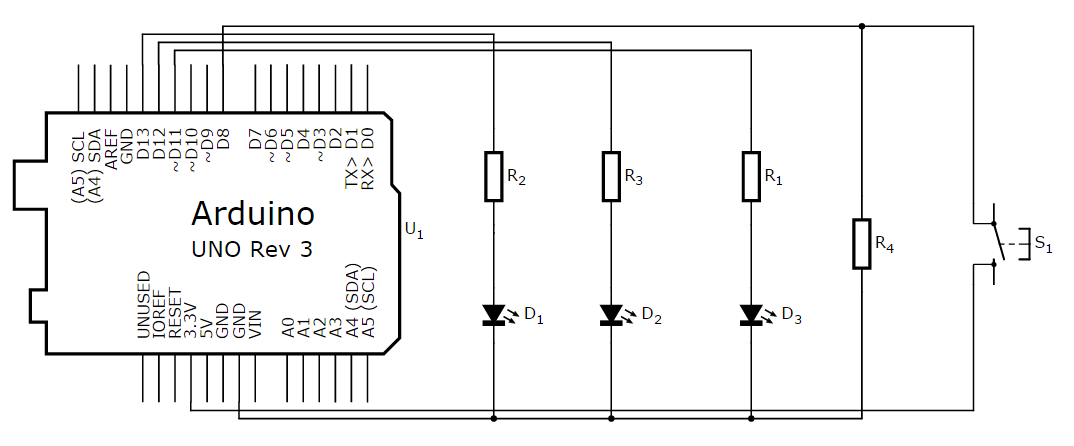
\includegraphics[scale=0.5]
  	{Fig/ArduinoCircuit.png}    
  	\caption{Schematic Circuit.}
\end{figure}

The R1, R2 and R3 resistors are rated 220 ohms, and are connected to the 13, 12 and 11 pins on the arduino respectively and then in series with them a led polarized to grown, the R4 resistor or Pull Down resistor is between the ground and the lecture of the 8th pin of the arduino, this for assurance that the read will be clear a logic 1 or a logic 0, without floating ground errors. The switch or button is connected between the 3.3 v pin of the arduino and the 8th pin for the logic lecture.
\subsection{Arduino}
Once you have mounted the circuit and connected to the Arduino, connect this to the computer, you must open the Arduino's Firmware folder in the Linux terminal and run the following commands:
\begin{enumerate}
\item \$ avr-gcc -Os -DF\_CPU=16000000UL -mmcu=atmega328p -c -o ArduinoInt.o ArduinoInt.c
\item \$ avr-gcc -mmcu=atmega328p ArduinoInt.o -o ArduinoInt
\item \$ avr-objcopy -O ihex -R .eeprom ArduinoInt ArduinoInt.hex
\item \$ avrdude -F -V -c arduino -p ATMEGA328P -P /dev/ttyACM0 -b 115200 -U flash:w:ArduinoInt.hex
\end{enumerate}
For this project it was mounted in a little box. See the Fig. \ref{Box}

\begin{figure}[h!]
 	\centering
  	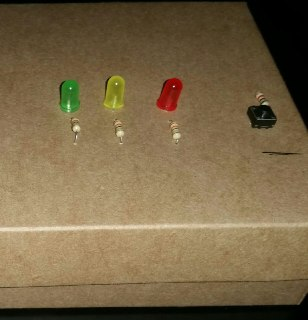
\includegraphics[scale=0.5]
  	{Fig/Box.jpg}    
  	\caption{Arduino and circuit Box.}
    \label{Box}
\end{figure}
Yo can push the button for see the LEDs animation, by default the animation is in Mode One, that means that the LEDs go to turn ON/OFF.
Then you can send a serial message with the following codes:
\begin{itemize}
\item 00: To select mode one, that are the ON/OFF mode.
\item 01: To select the mode two, that are the burst mode, this mode makes a LED burst, that means each LED go turn ON/OFF sequentially, one by one. 
\newline\newline Note: It is recommended to use the Arduino IDE and the tool Serial Monitor for sent the serial message.
\newline\newline Now you can push the button and enjoy the LEDs animation, and if change the mode, if you want.
\end{itemize}

\subsection{Arduino LKM}
For the LKM part you just have to compile it and insert it to the kernel.
IMPORTANT: Connect the arduino before loading the module.
\begin{enumerate}
\item Go to the program directory and locate the ArduinoLKM.c file and the Makefile.
\item Open a terminal there, and type  \emph{\$ make} to build the module.
\item Use the command  \emph{\$ sudo insmod ArduinoLKM.ko} to insert the module to the kernel, in this part a password entry will be prompt. Use your root password to gain super user privileges.
\item At this point the module is already loaded and you can modify his attributes at the /sys/Android/ttyACM0 directory this with a \emph{\$ cd /sys/Android/ttyACM0}
\item You can  \emph{\$ls} (list the configuration files),  \emph{\$echo} to all the configuration files but the ledStatus, and  \emph{\$cat} to all of them. Fig 7.
\item To unload the module a simple \emph{\$ sudo rmmod ArduinoLKM} will do.
\end{enumerate}
\begin{figure}[h!]
 	\centering
  	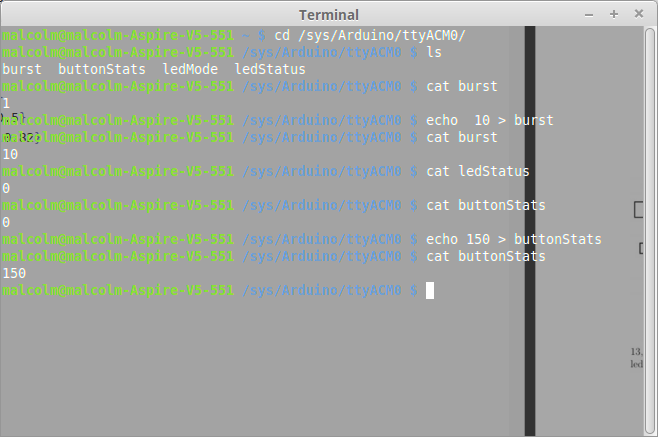
\includegraphics[scale=0.5]
  	{Fig/terminal.png}    
  	\caption{Terminal Commands Example.}
    \label{Box}
\end{figure}

%---------------------------------------
\section{Student Activity Log}
Include here the details of the activities performed by each of the students in this assignment.
Include one line per each activity, providing details like:
\begin{itemize}
\item Description of the activity.
\item Amount of time in hours/minutes spent on each activity.
\item Total amount of hours spent in the development of this project per student.
\item Use a time-sheet format (or tablet) to present this activity log.
\end{itemize}
\subsection{Arturo's Time-Sheet}
\begin{center}
\begin{tabular}{ |c|c|c| } 
 \hline
 Date & Task Description & Spent Time \\ 
 \hline\hline
  03/10/2016 & Installed the klinux headers and gcc-avr packages & 0.5 hours\\
 03/10/2016 & Read an article and make a "Hello World LKM" & 1.5 hours\\ 
  03/19/2016  & Documentation process start & 2 hours\\ 
   03/20/2016  & Create organization and repository on GitHub & 0.5 hours\\
   03/21/2016 &Investigation about LKM's&16 hours \\
   03/22/2016 &Investigation about LKM's&16 hours \\
   03/23/2016 &Investigation about C code for Arduino and av-gcc&16.5 hours \\
   03/24/2016 &Write the first version of firmware&16.5 hours\\
   03/25/2016 &Fix some bugs in the firmware&15 hours \\\
   03/26/2016 &Write the final version and complete the documentation&14.5 hours \\
 \hline
 & Total & 99 hours\\ 
 \hline
\end{tabular}
\end{center}
\subsection{Malcolm's Time-Sheet} 
\begin{center}
\begin{tabular}{ |c|c|c|} 
 \hline
 Date &  Task Description &  Spent Time \\ 
 \hline\hline 
 03/10/2016 & Installed the klinux headers and gcc-avr packages.& 0.5 hour\\
 03/10/2016 & Make the "Hello World LKM" & 1 hour \\
 03/19/2016 & Documentation process start & 2 hours\\ 
   03/21/2016 &Investigation about LKM's&16.5 hours \\
   03/22/2016 &Investigation about tty communication& 16.5 hours \\
   03/23/2016 &Investigation about tty communication& 16.5 hours \\
   03/25/2016 &Try to enable the communication between the programs&16 hours \\
   03/26/2016 &Fix and debug the code, complete the documentation&14.5 hours \\
  \hline
 & Total & 115.5 hours\\ 
 \hline
\end{tabular}
\end{center}

\section{Project final status}
The project could not be completed in its entirety, this because the Linux kernel module could not establish communication with the Arduino firmware. You can not directly access the serial port Arduino (ttyACM0) because there is already a driver module running on that port and can not be replaced.
About the Arduino, it can't change the amount of the repetitions from by the serial port, by default the repetitions is 1.

\subsection{Issues, Limitations and Challenges}
\begin{itemize}
\item The limited documentation on matters of creating Linux kernel modules, and the few code examples that have internal documentation explaining how it worked.
\item Trying to manipulate (read / write) files in the user space from the Linux kernel module, many of the references found indicated that this was not allowed. "The most common question asked in this don't-do-that category is, “How do I read a file from within my kernel module?” Most new kernel developers are coming from user-space programming environments or other operating systems where reading a file is a natural and essential part of bringing configuration information into a program. From within the Linux kernel, however, reading data out of a file for configuration information is considered to be forbidden. This is due to a vast array of different problems that could result if a developer tries to do this" \cite{LinuxJournal}

\item Reading the Arduino ports with C language and AVR-GCC compilers, because the major part of documentation was for Arduino language code. Because Arduino language is simplest and also all is documented. 
\end{itemize}
\subsection{Know Issues}
\begin{itemize}
\item Could not establish communication between the module Kernel Linux and Arduino, this because the LKM ought to manipulate user space files , which can not be done, the only documented way is through the use of an application running on user space, which according to the approach of the specification given in the project was not right.
\end{itemize}
\section{Conclusions, Suggestions and Recommendations.}
\begin{itemize}
\item Tools like the handler code versions is very useful, because in case of any failure in the new version allows us to return to a previous, plus the possibility of linking it to the storage service in the cloud, to share, and work together in a very easy way.
\item Sublime Text can be one of the better text editors, that should not make lack in the programmer's computer, for its flexibility and support for multiple programming languages, in addition to the vast amount of functionality adapted for this use.
\item 123D Circuits is a very practical tool for circuits simulation, provides a wide range of electronic elements, the simulation gives us the assurance that the circuit is good, to proceed to assemble it without breaking our devices.
\item Create Linux kernel Modules for Kernel 3.x is not easy, because it is relatively new (2011), and much of the information refers to older versions, especially the kernel version 2.x.
\item Create the firmware for the Arduino using pure C and avr-gcc compiler is very tedious, because there is little amount of information about how to do it. Apart from this internal documentation of the examples is too little.
\item The approach taken for the LKM of writing on the device file to manage the configuration parameters and the state of the circuit is not the best, this is because of the must of the must not of the kernel. It's recommended look for other approach to make this task.
\item It's important to separate the user space functions or programs and the kernel space, for all the power that it's within it.
\item For the project and the requirements purposes other approach that doesn't do much is the one that use the mayor number of the device to link it, this is because as far our research go this only create new tty ports and does not link a one that the O.S already mount.

\end{itemize}

%-------------------------------------------------------------------------------------------
%	References
%-------------------------------------------------------------------------------------------
\newpage
\begin{thebibliography}{10}
\bibitem{Molloy}
  D.  Molloy,
  \emph{"Writing a Linux Kernel Module — Part 1: Introduction"}
  derekmolloy.ie, 
  April 14th, 2015. [Online]. 
  Available: http://derekmolloy.ie/writing-a-linux-kernel-module-part-1-introduction/. 
  [Accessed: 20- Mar- 2016].
\bibitem{Henderson06}
  B. Henderson,
  \emph{"Linux LKM"},
  The Linux Documentation Project,
  2006. [Online]. 
  Available: http://www.tldp.org/HOWTO/Module-HOWTO/index.html 
  [Accessed: 20- Mar- 2016].
\bibitem{Salzman-Burian-Pomerantz}
  P. Salzman, M. Burian and O. Pomerantz, 
  \emph{"The Linux Kernel Module Programming Guide"},
  The Linux Documentation Project, 2007. 
  [Online]. Available: http://www.tldp.org/LDP/lkmpg/2.6/html/lkmpg.html.
  [Accessed: 27- Mar- 2016].
\bibitem{LinuxJournal}
  G.  Kroah-Hartman
  \emph{"Driving Me Nuts - Things You Never Should Do in the Kernel"}.
  Linux Journal,
  2005. [Online].
  Available: https://www.linuxjournal.com/article/8110?page=0,0.
  [Accessed: 26- Mar- 2016].  
\bibitem{Hartman07}
  G. Kroah-Hartman,
  \emph{"Linux kernel in a nutshell"}.
  Sebastopol,
  CA: O'Reilly, 2007,
  p. 16.
\bibitem{Ritchie}
  D. Ritchie, \emph{"The Development of C Language"}. 
  Murray Hill: Bell Labs, 1993,
  pp. 1-9.
\bibitem{Chin-Dav16a}
	A. Chinchilla and M. Davis, 
    \emph{"Creating a Linux Kernel Module (LKM) using C to interact with Arduino"},
    Overleaf.com, 2016. [Online].
    Available: https://www.overleaf.com/read/zcbqrvszmsrb.
    [Accessed: 26- Mar- 2016].
\bibitem{Chin-Dav16b}
  A. Chichilla and M. Davis,
  \emph{"LKMInvestigation/Linux-Kernel-Module"},
  GitHub, 2016. [Online].
  Available: https://github.com/LKMInvestigation/Linux-Kernel-Module.
  [Accessed: 26- Mar- 2016].
\end{thebibliography}
%--------------------------------------------------------------------------------------------

\end{document}